\subsubsection{17.01.15}
\begin{enumerate}
	\item Время начала и окончания собрания: 16:00 - 21:00
	
	\item Цели собрания:
	\begin{enumerate}
		\item Написать программу автономного периода, включающую в себя съезд с пандуса, заброс двух автономных шариков в 60см корзину и перемещение в зону парковки корзины 60см и 90см.
		
		\item Разобраться, как работает ИК-датчик.
		
		\item Написать программу автономного периода, в которой робот будет ориентироваться по ИК-датчику, включающую в себя заброс двух автономных шариков в центральную корзину(для старта из зоны парковки).
		
		\item Разобраться, как работает ИК-датчик.
		
		\item Написать программу автономного периода, в которой робот будет ориентироваться по ИК-датчику, включающую в себя заброс двух автономных шариков в центральную корзину (для старта из зоны парковки).
	\end{enumerate}
	\item Проделанная работа:
	\begin{enumerate}
		\item Было решено осуществить завоз двух корзин в зону парковки по следующему алгоритму: после заброса автономных шариков в 60см корзину отвозим сначала ее, затем разворачиваемся, едем к 90см корзине и отвозим ее.
		
		\item Программа была написана и протестирована. Результат положительный: робот способен проделать все действия за 30 секунд.
		
		\item  ИК-датчик был установлен сзади на робота.
		
		\item  ИК-датчик был установлен сзади на робота.

		\begin{figure}[H]
			\begin{minipage}[h]{0.2\linewidth}
				\center  
			\end{minipage}
			\begin{minipage}[h]{0.6\linewidth}
				\center{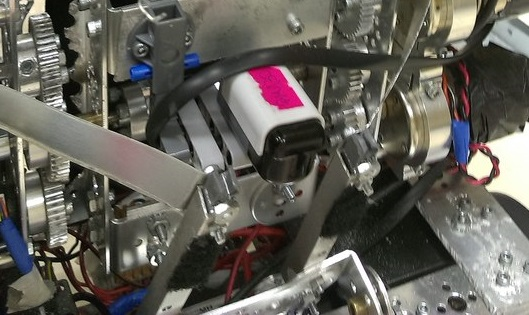
\includegraphics[scale=0.3]{days/17.01.15/images/01}}
				
				\caption{ИК-датчик на роботе}
			\end{minipage}
		\end{figure}
		
		\item Для освоения ИК-датчика были написаны две простейшие программы: первая - выводить на экран показания ИК-датчика, вторая - вращаться вокруг своей оси пока ИК-излучатель не будет в определенном положении относительно робота.  
		
		\item Программа заброса двух шариков в центральную корзину была написана по следующему алгоритму: сначала определяем положене центральной корзины, если корзина прямо перед роботом, то едем задним ходом по прямой и забрасываем шарики, если сбоку, то делаем поворот в сторону корзины так, чтобы робот мог проехать между корзиной и одним из пандусов. Далее едем прямо, пока корзина не будет перпендикулярна роботу, затем поворачиваем так, чтобы она была прямо перед роботом. Затем подъезжаем к корзине и забрасываем шарики.
		
		\item Программа была написана и протестирована. Результат отрицательный: если ИК-излучатель находится сбоку от робота, то робот поворачивает и едет по прямой, не останавливаясь, даже когда излучатель находится перпендикулярно относительно датчика.   
	\end{enumerate}
	\item Итоги собрания:
	\begin{enumerate}
		\item Программа автономного периода с завозом двух корзин в зону парковки написана.
		
		\item ИК-датчик освоен.
		
		\item Для освоения ИК-датчика были написаны две простейшие программы: первая - выводить на экран показания ИК-датчика, вторая - вращаться вокруг своей оси пока ИК-излучатель не будет в определенном положении относительно робота.  
		
		\item Программа заброса двух шариков в центральную корзину была написана по следующему алгоритму: сначала определяем положене центральной корзины, если корзина прямо перед роботом, то едем задним ходом по прямой и забрасываем шарики, если сбоку, то делаем поворот в сторону корзины так, чтобы робот мог проехать между корзиной и одним из пандусов. Далее едем прямо, пока корзина не будет перпендикулярна роботу, затем поворачиваем так, чтобы она была прямо перед роботом. Затем подъезжаем к корзине и забрасываем шарики.
		
		\item Программа была написана и протестирована. Результат отрицательный: если ИК-излучатель находится сбоку от робота, то робот поворачивает и едет по прямой, не останавливаясь, даже когда излучатель находится перпендикулярно относительно датчика.   
	\end{enumerate}
	\item Итоги собрания:
	\begin{enumerate}
		\item Программа автономного периода с завозом двух корзин в зону парковки написана.
		
		\item ИК-датчик освоен.
		
		\item Прграмма заброса автономных мячей в центральную корзину не написана.
	\end{enumerate}
	\item Задачи для последуюших собраний:
	\begin{enumerate}
		\item Доделать программу забрасывания двух автономных мячей в центральную корзину.
		
		\item Тренироваться в управлении роботом.
	\end{enumerate}
\end{enumerate}
\fillpage